%------------------------------------------------------------------------------
%	MDPS
%------------------------------------------------------------------------------


\subsection{\acrfull{MDP}} \label{mdpSec}

The problem of optimal stochastic control is usually handled using an \gls{MDP}, which provides a principled mathematical methodology that can address the uncertainties of planning optimum inspection and maintenance strategies,  including uncertain action outcomes and exact observations. The theory behind \glspl{MDP}, together with further concepts that will not be covered in the current work, like \glsxtrfullpl{SMDP}, State Augmentation, etc, has been analyzed in depth in many papers, e.g. \cite{papakonstantinou2014planning1}. However, a basic elaboration on \glspl{MDP} and \glsxtrfullpl{POMDP} will be made, in order to build a foundation for the more advanced concepts in the following sections.\\

The basic components of an \gls{MDP} are the Environment and the Agent, while it can  fully described by the tuple:

$$\langle \ccal{S,A,P,R}, \gamma \rangle$$

where, 

\begin{equation*}
    \begin{array}{lll}
        \ccal{S} & : & \text { the finite set of states } \\ 
        \ccal{A} & : & \text { the finite set of actions } \\ 
        \ccal{P} & : & \text { the state probability matrix } \\ 
        \ccal{R} & : & \text { the reward function } \\ 
        \gamma & : & \text{ a discount factor for the future rewards}
    \end{array}
\end{equation*}

At each decision step $t$, the decision-maker, i.e. the agent, observes the current state $s_t \in \ccal{S}$, takes an action $a_t\in \ccal{A}$, receives a reward $R_t(s_t, a_t)\in \ccal{R}$ and moves to the next state $s_{t+1}\in \ccal{S}$ based on the environment's transition dynamics. This procedure is displayed in Figure \ref{RLflow}. According to the so-called Markov property, the next state, $s_{t+1}$, depends only on the current state, $s_t$, and the chosen action, $a_t$, regardless from the preceding history of states and actions. The sequence of actions followed by the agent, defines its policy, $\pi$, that can be either deterministic or stochastic, meaning that a policy can map states to actions or states to probability mass (or density) functions, respectively.

\begin{figure}[H]
    \centering
	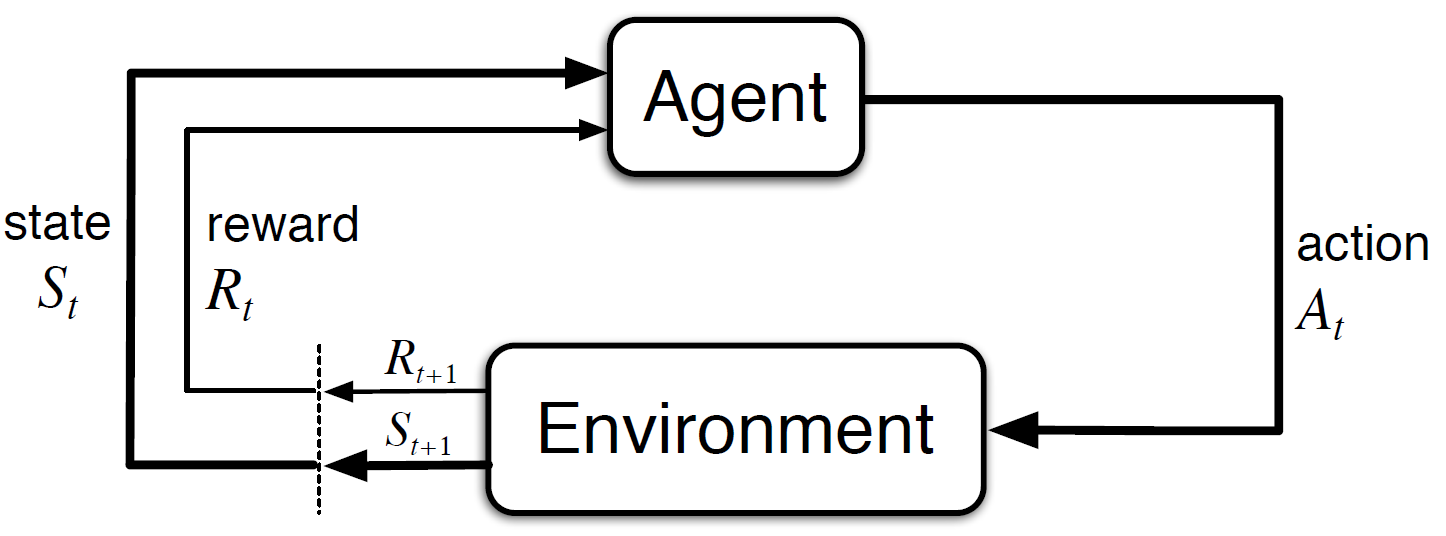
\includegraphics[width=0.65\linewidth]{Figures/RLclassicFig.png}
	\caption{The agent-environment interaction in an \gls{MDP} \cite{sutton2018reinforcement}}
	\label{RLflow}
\end{figure}


The ultimate goal of an optimal policy is to maximize the sum of the discounted rewards, i.e. the total return, $G_t$, of the chosen actions, which is given by the following formula:

\begin{equation}
    G_{t}=R(s_t, a_t)+\gamma\, R(s_{t+1}, a_{t+1})+\gamma^2\,R(s_{t+2}, a_{t+2})+\ldots= \sum_{i=t}^{T} \gamma^{i-t}\, R(s_i, a_i)  \label{expReturn}
\end{equation}

It should be noted that the total return is not deterministic, owing to the problem being stochastic. Thus, accounting for all future state-action pairs, the action-value function, $Q^{\pi}(s_t, a_t)$ is defined as the expected return\footnotemark over both $\ccal{S}$ and $\ccal{A}$ sets (Equation \ref{Qfunc}).

\begin{equation}
    Q^{\pi}(s_t, a_t) = \mathbb{E}_{s_t, a_t} \left[ G_t \mid s_t, a_t \right] \label{Qfunc} 
\end{equation}

It should be noted that the notation $\mathbb{E}$ corresponds to the expected value, i.e. the mean, while the variables over which it is computed, are denoted as the subscripts.\\

Decomposing $Q^{\pi}$ into the immediate reward plus the discounted value of the successor state, leads to the following recursive form:

\begin{equation}
    Q^{\pi}(s_t, a_t)=R(s_t, a_t) + \mathbb{E}_{s_{t+1}, a_{t+1}} \left[\gamma \, Q^{\pi}(s_{t+1},a_{t+1}) \mid s_t, a_t\right]
\end{equation}

The state-value function $V^{\pi}(s_t)$ is defined in a similar way, corresponding to the expected return starting from state $s_t$ and following policy $\pi$.

\begin{equation}
    V^{\pi}(s_t)=\mathbb{E}_{a_t} \left[ G_{t} \mid s_t \right] 
\end{equation}

Since the state-value function is stochastically defined for all possible actions of policy $\pi$, it takes the form:

\begin{equation}
    V^{\pi}(s_t)=\mathbb{E}_{a_t}\left[Q^{\pi}(s_t, a_t)\right]
\end{equation}

\newpage

For any \gls{MDP} there exists an optimal policy $\pi_{*}$ that achieves the optimal state and action-state value function. These are formulated through the Bellman Optimality Equation as follows:

\begin{gather}
    V^*(s_t) = \max _{a_t\in\ccal{A}} \left[ R(s_t,a_t) + \gamma \sum _{s_{t+1}\in \ccal{S}} \prob{s_{t+1}\mid s_t, a_t} \, V(s_{t+1}) \right] \label{optimalV}\\
    Q^* (s_t,a_t) = R(s_t, a_t) + \gamma \sum_{s_{t+1}\in \ccal{S}} \prob{s_{t+1}\mid s_t, a_t}\, \underset{a_{t+1}}{\text{max}} \, Q(s_{t+1},a_{t+1})
\end{gather}

The symbol $\prob{\cdot}$ corresponds to the probability of a quantity; a notation that will be used for the rest of the thesis.\\

When the optimal action-state value function is known, the optimal policy is known, thus the \gls{MDP} is solved. Since the Bellman Optimality Equation is non-linear, it is often solved using \gls{DP} (value iteration, policy iteration), or algorithms like Q-learning and SARSA (both will be presented in Section \ref{rlSec}).\\

A considerable disadvantage of using \glspl{MDP} for a sequential decision problem is the curse of dimensionality, as with an increase in the state-space, the computational cost grows exponentially. Therefore, in the existing literature, there are mostly attempts that choose discrete deterioration states instead of continuous, e.g. \cite{andersen2021numerical}, \cite{compare2018markov}.

%------------------------------------------------------------------------------
%	POMDPs
%------------------------------------------------------------------------------


\subsection{\acrfull{POMDP}} \label{pomdpSec}

A significant aspect in the exploitation of the ever-increasing available observation data is the degree of confidence the decision-maker has in the received input. This issue is undoubtedly connected with uncertainties regarding various environmental and loading conditions, modelling errors, inefficient measuring systems or inaccuracies in the information transmission network \cite{schobi2016maintenance}. This is why, more often than not, models based on \glspl{MDP} are limited by the need of perfect observations, leading to their extension to \glspl{POMDP}, which take into consideration the partial observability of the systems' information in order to approach the optimal sequence of maintenance decisions based on uncertain structural data. In these cases, when the states are not fully observable, at each decision step the agent gets a belief, $\boldsymbol{b}$, over the states of the system. Since the Markov property still holds, this probability distributions over $\ccal{S}$ is sufficient to describe the history of actions and observations. Starting with an initial belief, $\boldsymbol{b_t}$, the agent takes an action, $a_t$, but instead of receiving the new state, gets an observation $o_{t+1}\in \ccal{\Omega}$, with which the belief is updated, using Bayesian principles.

\begin{align}
    b(s_{t+1}) &= \prob{s_{t+1}\mid o_{t+1}, a_t, \boldsymbol{b_t}} \nonumber \\
    &= \cfrac{\prob{o_{t+1}\mid s_{t+1}, a_t}}{\prob{o_{t+1}\mid \boldsymbol{b_t},a_t}} \sum _{s_t \in \ccal{S}} \prob{s_{t+1}\mid s_t, a_t}\, b(s_t) \label{discBeliefEq}
\end{align}

In a similar notion with \glspl{MDP} and assuming that the beliefs are the states of this environment, Equation \ref{optimalV} can be rewritten for \glspl{POMDP}.

\begin{equation}
    V^*(\boldsymbol{b_t}) = \underset{a_t\in \ccal{A}}{\text{max}} \left[ \sum _{s_t\in\ccal{S}} b(s_t) \, R(s_t, a_t) + \gamma \sum _{o\in \ccal{\Omega}} \prob{o\mid \boldsymbol{b},a) V(\boldsymbol{b_{t+1}}}\right]
\end{equation}

\glspl{POMDP} have been used in many cases for infrastructure maintenance in the existing literature (\cite{corotis2005modeling}, \cite{nguyen2019joint}) often along with point-based algorithms (\cite{papakonstantinou2014planning2}, \cite{papakonstantinou2018pomdp}, \cite{andriotis2021value}, \cite{morato2022optimal}, \cite{morato2019pomdp}) demonstrating that they can model more efficiently complex decision problems outperforming heuristic-based policies. However, they face limitations when it comes to the solution of large action- and state-spaces, and even greater ones in the case of continuous state spaces. The most significant difficulty lays on the updating of the belief, with Equation \ref{discBeliefEq} (which corresponded to discrete spaces) taking the following~form:

\begin{equation}
    b^{\prime}(s_{t+1}) = \prob{s_{t+1} \mid o_{t+1}} \propto \prob{o_{t+1} \mid s_{t+1}, a_t} \, \int _{s_t} \prob{s_{t+1} \mid s_t, a_t} \, b(s_t) \mathrm{d}s_t \label{contBeliefEq}
\end{equation}

Because the integral of Equation \ref{contBeliefEq} can not be calculated in a closed form, many researchers have attempted to use other mathematical ways that work around this issue (\cite{dallaire2009bayesian}, \cite{brooks2006parametric}, \cite{zhou2010solving}). This updating of the belief can be broken down into two steps, the \textit{transition step}, during which the belief propagates in time according to a predefined conditional probability distribution \cite{morato2022optimal}:

\begin{equation}
    b(s_{t+1}) = \int _{s_t} \prob{s_{t+1} \mid s_t, a_t} \, b(s_t) \mathrm{d}s_t
\end{equation}

and the \textit{estimation step}, with the belief now updating based on obtained evidence by means of Bayes' rule:

\begin{equation}
    b^{\prime}(s_{t+1}) = \prob{s_{t+1} \mid o_{t+1}} \propto \prob{o_{t+1} \mid s_{t+1}, a_t} \,b(s_{t+1})
\end{equation}

These drawbacks and difficulties of \glspl{POMDP} led to the need of developing an \gls{RL} or \gls{DRL} methodology, capable of tackling them.

%------------------------------------------------------------------------------
%	RL
%------------------------------------------------------------------------------


\subsection{\acrfull{RL}} \label{rlSec}

\gls{RL} is often an advantageous technique to deal with sequential decision optimization, especially when knowledge about the system is uncertain or unknown. Indeed in the existing literature there are even examples that tackle optimal maintenance planning in the absence of a deterioration model \cite{durango2004maintenance}. The agent interacts directly with the environment by taking actions and adjusts the policy based on the information received back, aiming to identify the optimal one. \\

\gls{RL} algorithms are divided into two main categories, model-based and model-free. In the former group, e.g. \gls{DP} (policy iteration, value iteration), the model must provide state transition probabilities and expected rewards for every state-action pair in order to identify the optimal policy, whereas algorithms in the latter category, such as \gls{TD} learning, SARSA, Q-learning, rely on real samples from the environment, which is a feature that makes them applicable in various different cases. Both model-based and model-free approaches were tested along with Q-learning in \cite{zhang2021model}, for a problem of maintenance optimization, with the system's discrete state transitions being defined through the assumed degradation model. \\

A second major distinction between \gls{RL} algorithms, is the one among on-policy and off-policy. In on-policy learning the $Q(s, a)$ function is learned through actions of the current policy, $\pi$, while in off-policy learning, it is learned while taking different/random actions. Namely, SARSA is an on-policy algorithm, that updates the state-action value function as follows:

\begin{equation}
    Q(s_t, a_t) \leftarrow Q(s_t,a_t) + \alpha \, \left( R(s_t, a_t) + \gamma \, Q(s_{t+1}, a_{t+1}) - Q(s_t, a_t) \right)
\end{equation}

where $a_{t+1}$ is the action taken according to policy $\pi$.\\

On the other hand, Q-learning is an off-policy learning algorithm, that updates the state-action value function in the following way:

\begin{equation}
    Q(s_t, a_t) \leftarrow Q(s_t,a_t) + \alpha \, \left( R(s_t, a_t) + \gamma \, \underset{a_{t+1} \in \ccal{A}}{\text{max}}Q(s_{t+1},a_{t+1}) - Q(s_t, a_t) \right)
\end{equation}

where $a_{t+1}$ can be any of the possible actions.\\

In Q-learning, the value functions $Q$ for any state-action pair are stored in a table, and they are updated by interacting with the environment, i.e. taking actions and receiving rewards. In order to explore every possible action, hence, every unknown area of the Q-table, usually an $\epsilon$-greedy policy is used, in order to balance out exploration and exploitation. More specifically, the agent will exploit the already known Q-values, or explore, picking an action at random, based on the following rule:

\begin{equation}
    a_t = 
    \begin{cases} 
        \underset{a_t\in \ccal{A}}{\text{max}}Q(s_t, a_t) & \text{with probability } 1-\epsilon \\
        \text{random } a_t \in \ccal{A} & \text{with probability } \epsilon
    \end{cases}
\end{equation}

In \cite{memarzadeh2019model}, a customized version of Q-learning is introduced, namely "\textit{safe Q-learning}", that includes a model-based safe exploration for near-optimal management of infrastructure, in order to decrease the variance induced by choosing random actions (exploring).\\

However, there are two main limitations in the classic Q-learning approach, which are (1) the curse of dimensionality when the state- and action-space are large, and (2) the inability of this algorithm to visit all states, hence, to estimate the Q-values for the whole table. 


%------------------------------------------------------------------------------
%	DRL
%------------------------------------------------------------------------------


\subsection{\acrfull{DRL}}

To tackle the aforementioned limitations, the Q-function is approximated through a \acrfull{DNN}. This way, the state-action value function is reparameterized, and is now expressed in terms of parameters $\theta$, in order to alleviate the computational cost and instabilities that large state- and action-spaces~cause. \\

\subsubsection{\acrfull{DQN}}

The state, $s_t$ is given as an input to the \gls{DNN}, and by using a suitable number of inner layers and activation functions, it outputs the action-state value function, $Q(s_t, a_t\mid \theta)$, for every $a_t \in \ccal{A}$. The parameters, $\theta$, i.e. the Q-network weights, are adjusted in every iteration of the agent's training in order to minimize a sequence of loss functions that are given by the following equation:

\begin{equation}
    L(\theta) = \mathbb{E}_{s_t, a_t}\left[ \left( (y_t - Q(s_t, a_t\mid \theta ) \right) ^2 \right]
\end{equation}

with $y_t$ being the target for decision step $t$,

\begin{equation}
    y_t = \mathbb{E}_{s_{t+1}}\left[ R(s_t, a_t) + \gamma \, \max _{a_{t+1}} Q(s_{t+1}, a_{t+1}\mid \theta ^-) \mid s_t, a_t \right] \label{targetQ}
\end{equation}

In order to stabilize the learning process, tuples of $(s_t, a_t, R(s_t, a_t), s_{t+1})$ are being stored in a replay buffer and are then used in batch training the \gls{DQN} according to the following gradient:

\begin{equation}
    \nabla_{\theta} L\left(\theta \right)=\mathbb{E}_{s_t, a_t}\left[\left(R_t(s_t,a_t)+\gamma \max _{a_{t+1}\in \ccal{A}} Q\left(s_{t+1}, a_{t+1} \mid \theta ^- \right) -Q\left(s_t, a_t \mid \theta \right)\right) \nabla_{\theta} Q\left(s_t, a_t \mid \theta \right)\right] \label{gradLoss}
\end{equation}

Each tuple of the experience replay is potentially used in many weight updates, which leads to the use of non-consecutive uncorrelated samples, hence, to the reduction of the variance through the updates. Additionally, as it is shown in Equations \ref{targetQ}, \ref{gradLoss}, a target network is used, with parameters $\theta ^-$. This target network takes the values of the original one with a delay, which contributes to the stability of the training.\\

Various examples exist in the literature, using \gls{DQN} including different \glspl{DNN} to approximate the value functions. In the initial coupling of \gls{RL} and \gls{DL} by DeepMind \cite{mnih2013playing}, \glspl{CNN} were used in order to decompose the Atari's screen into a rectangular grid that was fed into the network. Similarly, a \gls{DRL} framework for optimal maintenance, again with a \gls{CNN} is developed in \cite{wei2020optimal}. Moreover, in both \cite{hausknecht2015deep} and \cite{meng2021memory}, \glspl{RNN} are used for the policy optimization while in a partially observable environment. Finally, an \gls{ANN} is used in \cite{egorov2015deep} in order to tackle the two-dimensional state-space limitation, existing in cases when \glspl{CNN} or \glspl{RNN} were chosen instead. This approach was followed in \cite{rocchetta2019reinforcement}, too, as well as in \cite{yang2022adaptive} where an \gls{ANN} was used both for the multi-component system's maintenance but also for the creation of a surrogate model.



\subsubsection{\acrfull{DDQN}}

It is known that standard \gls{DQN} suffers from an overestimation problem for the action values in noisy environments, thus, an even more stable algorithm is \gls{DDQN} that uses both the target and the original network in the calculation of $y_t$,  in particular:

\begin{equation}
    y_{t}=R(s_{t}, a_{t})+\gamma \,Q\left(s_{t+1}, \arg \max Q\left(s_{t+1}, a_{t+1} \mid \theta \right) \mid \theta^- \right)
\end{equation}

In \cite{zhang2020deep} a \gls{DDQN} is used for the maintenance planning of a stochastically deteriorating system, accounting also for the dependency between its multiple components. \gls{DDQN} is thoroughly explained in \cite{van2016deep}.

\subsubsection{\acrfull{A2C}}

Another common approach in both \gls{RL} and \gls{DRL} is to instead of interacting with value functions, change directly the policy, $\pi$. In the case of \gls{DRL}, when a \gls{DNN} is used to approximate $\pi$, the training is done through the gradient:

\begin{equation}
    \nabla _{\theta} J(\theta) = \mathbb{E}_{s_t,a_t}\left[ \sum _{t\geq 0} \nabla _{\theta} \log \pi (a_t \mid s_t, \theta) \, Q(s_t,a_t) \right] \label{polGrad}
\end{equation}

where $J(\theta)$ is the objective function, i.e. 

\begin{equation}
    J(\theta)=\sum _{t\geq 0} \gamma ^t \, R(s_t, a_t)
\end{equation}

One way to reduce the variance and improve policy gradient methods is by subtracting a baseline from the Q-function. This is why the advantage value is being introduced:

\begin{equation}
    A(s_t, a_t) = Q(s_t, a_t) - V(s_t) \label{adv}
\end{equation}

corresponding to how much better a specific action is, compared to the average, general action at the given state.\\

In order to compute all terms in Equation \ref{polGrad}, the policy gradient requires also an estimation of a value function. This issue led to the creation of the so-called Actor-Critic methods, which use a value approximator (critic) to train the parameters of the policy approximator (actor). Two \glspl{DNN} are employed, one for each of the two approximators (actor-network, critic-network), with the latter being used for the V-function estimation, since Equation \ref{adv} can be rewritten through the Bellman equation as follows:

\begin{equation}
    A(s_t, a_t) = R(s_t, a_t) + \gamma \, V(s_{t+1}) - V(s_t)
\end{equation}

\newpage

This leads to the \gls{A2C} algorithm, which aims to the minimization of:

\begin{align}
    \nabla _{\theta} J(\theta) &= \mathbb{E}_{s_t,a_t}\left[ \sum _{t\geq 0} \nabla _{\theta} \log \pi (a_t \mid s_t, \theta) \, \left( R(s_t, a_t) + \gamma \, V(s_{t+1}) - V(s_t) \right) \right] \nonumber \\
    &= \mathbb{E}_{s_t,a_t}\left[ \sum _{t\geq 0} \nabla _{\theta} \log \pi (a_t \mid s_t, \theta) \, A(s_t,a_t) \right]
\end{align}

\subsubsection{\acrfull{PPO}}

In order to avoid destructively large policy updates in policy gradient algorithms, the trust region methods were developed. In particular, the \gls{TRPO} algorithm, aims to maximize the "surrogate" objective function, under the constraint that the \gls{KL} divergence between the old and new policy is less than a constant $\delta$.

\begin{gather}
    \underset{\theta}{\text{maximize }} \, \mathbb{E}_t \left [ \cfrac{\pi_{\theta}(a_t \mid s_t)}{\pi _{\theta _{\text{old}}}(a_t \mid s_t)} A_t\right]\\
    \text{with } \quad \mathbb{E}_t\left [ \text{KL} \left[ \pi_{\theta_{\text{old}}}(\cdot \mid s_t), \pi_{\theta}(\cdot \mid s_t) \right ] \right] \leq \delta
\end{gather}

or, using a penalty term instead of a constraint:

\begin{equation}
    \underset{\theta}{\text{maximize }} \, \mathbb{E}_t \left [ \cfrac{\pi_{\theta}(a_t \mid s_t)}{\pi _{\theta _{\text{old}}}(a_t \mid s_t)} A_t -\beta \, \text{KL} \left [ \pi_{\theta_{\text{old}}}(\cdot \mid s_t), \pi_{\theta}(\cdot \mid s_t) \right] \right]\\    
\end{equation}

An improvement to \gls{TRPO} is the \gls{PPO} algorithm. Although, an in depth description of this method is presented in \cite{schulman2017proximal}, a brief reference to its main steps/equations will be also included here.\\

Denoting the probability ratio,

\begin{equation}
    r_t(\theta) = \cfrac{\pi_{\theta}(a_t \mid s_t)}{\pi _{\theta _{\text{old}}}(a_t \mid s_t)}
\end{equation}

the \gls{TRPO} "surrogate" objective becomes:

\begin{equation}
    L^{C P I}(\theta)=\mathbb{E}_{t}\left[\frac{\pi_{\theta}\left(a_{t} \mid s_{t}\right)}{\pi_{\theta_{\text {old }}}\left(a_{t} \mid s_{t}\right)} A_{t}\right]=\mathbb{E}_{t}\left[r_{t}(\theta) A_{t}\right]
\end{equation}

The superscript $CPI$ refers to conservative policy iteration, while the maximization of $L^{C P I}$ would cause large policy updates. Therefore, the objective needs to be adjusted so as to penalize policy changes that move $r_t(\theta)$ away from 1. Thus, the clipped surrogate objective is considered instead:

\begin{equation}
    L^{C L I P}(\theta)=\mathbb{E}_{t}\left[\min \left(r_{t}(\theta) A_{t}, \operatorname{clip}\left(r_{t}(\theta), 1-\epsilon, 1+\epsilon\right) A_{t}\right)\right]
\end{equation}

The term, $\operatorname{clip}\left(r_{t}(\theta), 1-\epsilon, 1+\epsilon\right)A_t$, modifies the surrogate objective by clipping the probability ratio, not allowing it to move outside the interval $\left[ 1-\epsilon, 1+\epsilon \right]$.\\

\gls{PPO} is used to optimize the maintenance of renewable energy systems in \cite{pinciroli2022optimization}.

\subsubsection{Other \acrfull{DRL} algorithms}

Regarding different \gls{DRL} algorithms, \gls{DDPG} is used in \cite{chen2021deep}, which is an actor-critic algorithm that enables the modeling of a continuous deterioration state-space. Additionally, the development of a new algorithm, namely \gls{DCMAC}, is presented in \cite{andriotis2019managing} that aims for the optimal maintenance in multi-component systems with high dimensional action- and state-spaces. Lastly, in order to address challenges regarding stochastic optimal control, such as the curse of dimensionality in large spaces, the curse of history, and the environment uncertainties/stochasticity, \gls{DDMAC} is introduced in \cite{andriotis2021deep}.

%------------------------------------------------------------------------------
%	BMU
%------------------------------------------------------------------------------


\subsection{\acrfull{BMU}} \label{bmuSec}

As it has already been mentioned, in the current project, the problem of optimal stochastic control will be combined with the notion of \gls{BMU}. To be more precise, model updating constitutes an inverse problem, meaning that, instead of knowing beforehand the exact parameters of a model to calculate its response, observations of the system's behavior are used in order to update or calibrate the unknown system properties. This technique can efficiently tackle the fact that many system parameters are not deterministic, but stochastic. Additionally, in most cases the deterioration of an existing structure can not be modeled accurately, with a Gamma process e.g. like in \cite{zhang2020deep}, \cite{andriotis2019managing}, \cite{zhou2022maintenance} (this type of deterioration will be covered in depth in Section \ref{detProcsSec}) or generally a relationship of the form $D(t) = A\, t^B$ for the damage, $D(t)$, over time, $t$, e.g. like in \cite{kamariotis2022value}. Therefore, an updating procedure can be useful in defining its properties during its whole service life. An extensive review on model updating about damage assessment, including \gls{BMU} is presented in \cite{simoen2015dealing}.\\

It should be mentioned that, a detailed and instructive example on how to account for a structure's deterioration through \gls{BMU} is presented in \cite{kamariotis2022value}. In that research, aiming to quantify the \gls{VoI}, periodic inspections are made, and the obtained observation are used in the updating of the system's parameters as well as its structural reliability. A heuristic based approach was followed regarding the life-cycle optimization.

\newpage

From a more technical standpoint, Bayesian Inference is performed using Bayes' Theorem, which, assuming that $\boldsymbol{\theta}$ are the parameters of interest and $\boldsymbol{D}$ are the observations, takes the form: 

\begin{equation}
    \prob{\boldsymbol{\theta}\mid \boldsymbol{D}} = \cfrac{\prob{\boldsymbol{D}\mid \boldsymbol{\theta}} \, \prob{\boldsymbol{\theta}}}{\prob{\boldsymbol{D}}} \label{bayesTheorem}
\end{equation}

where,

\begin{equation*}
    \begin{array}{lll}
        \boldsymbol{\theta} & : & \text{ the vector of the parameters of interest} \\ 
        \boldsymbol{D} & : & \text { the vector of observations} \\ 
        \prob{\boldsymbol{\theta}} & : & \text { the prior distribution } \\ 
        \prob{\boldsymbol{D}\mid \boldsymbol{\theta}} & : & \text { the likelihood function of the parameters } \boldsymbol{\theta}\\ 
        \prob{\boldsymbol{D}} & : & \text{ the evidence}\\
        \prob{\boldsymbol{\theta} \mid \boldsymbol{D}} & : & \text{ the posterior distribution of } \boldsymbol{\theta}
    \end{array}
\end{equation*}

Analyzing each factor involved in Equation \ref{bayesTheorem}:

\begin{itemize}
    \item \textbf{Prior distribution}\\
        The prior distribution $\prob{\boldsymbol{\theta}}$ corresponds to the initial hypothesis about the system's parameters. It is an uninformed estimation of them, e.g. if only the upper and lower bounds are known, a Uniform distribution among these bounds will be used.
    \item \textbf{Likelihood function}\\
        The likelihood function describes the degree of agreement between the observations $\boldsymbol{D}$ and the output/result of the actual model, computed deterministically using the existing knowledge for parameters $\boldsymbol{\theta}$
    \item \textbf{Evidence function}\\
        The evidence function acts as a normalizing constant in Bayes Theorem. This way the integral of the posterior distribution sums up to 1. Because the evidence is independent from parameters $\boldsymbol{\theta}$, it does not affect the shape of the posterior distribution, hence, it can be written:
        \begin{equation}
            \prob{\boldsymbol{\theta} \mid \boldsymbol{D}} \propto \prob{\boldsymbol{D} \mid \boldsymbol{\theta}} \, \prob{\boldsymbol{\theta}}
        \end{equation}
    \item \textbf{Posterior distribution}\\
        The posterior distribution is the updated distribution of parameters $\boldsymbol{\theta}$ with the use of the observed response data. 
\end{itemize}

A challenge lays on the sampling of the posterior distribution, because it can not be expressed in a closed form, but only implicitly, point-wise, using a \gls{MC} approach. To overcome this obstacle, many sampling methods have been developed, in order to approximate $\prob{\boldsymbol{\theta} \mid \boldsymbol{D}}$. An in-depth overview of three popular sampling methods, namely \gls{MCMC}, \gls{TMCMC} and \gls{SMC} is presented in \cite{lye2021sampling}. Two of the most well-known \gls{MCMC} algorithms are Metropolis-Hastings and Gibbs sampling. However, they often fail to converge to the posterior distribution, especially for continuous model parameters. Therefore, more efficient algorithms have been developed and are widely used, such as \gls{HMC}, and an even more advanced variation of it, \acrfull{NUTS}. \gls{NUTS} tends to be significantly efficient, thanks to its stability and the fact that it does not need hand-tuning of hyper-parameters by the user. A brief elaboration on \gls{NUTS} is presented in Section \ref{nutsSec}, whereas an in-depth presentation of it, and its many variations, is included in \cite{hoffman2014no}. \\

Concluding, the stochastic nature of this problem, and the inability to know the exact value for the parameters of interest at every decision step, comes to highlight the need of \gls{POMDP}, where the belief, $\boldsymbol{b_t}$ at every $t$, will correspond to the posterior distribution, after having incorporated the observations $D$.\\

%------------------------------------------------------------------------------
%	DETERIORATION PROCESSES
%------------------------------------------------------------------------------


\subsection{Deterioration Processes} \label{detProcsSec}

As elaborated thoroughly in \cite{van2020stochastic} and \cite{van2009survey}, the uncertainty associated with the evolution of degradation over time is an important consideration for the optimisation of maintenance. The commonly used \gls{RVD}, where the rate of degradation\footnotemark is random, can not capture the temporal variability of the degradation, which is why a \gls{SPD} model is usually adopted. An efficient modelling option would be the Brownian motion with a drift. A stochastic process that has been applied successfully in a plethora of fields (e.g. exchange value of shares, movement of small particles in fluids, etc), however in the current application fails to perform due to the fact that it can alternately increase and decrease, which is not the case for a structure's performance, which monotonically decreases. Therefore, more often than not, the stochastic process chosen for the modelling of an engineering system's deterioration is the Gamma process. It is a stochastic process with independent non-negative increments that have a gamma distribution with identical scale parameter and time-dependent shape parameter. This choice has been proven suitable to model gradual damage monotonically accumulating over time applicable to a variety of problems e.g. wear, fatigue, corrosion, crack growth, erosion, consumption, creep, swell, etc \cite{van2020stochastic}.\\

\footnotetext{For a degradation in the form of $A\,t^B$, linear parameter $A$ is known as the rate of degradation, while $B$ is the non-linear trend of the degradation law. Usually, $A$ reflects the variability in a large population of similar components.}

\newpage

At every step $t$, the damage $d$ follows a Gamma distribution with shape $v(t) > 0$ and scale $u > 0$. Mathematically, its \gls{PDF} is given by:

\begin{equation}
    \mathrm{Ga}(d \mid v(t), u) = \cfrac{u^v(t)}{\mathrm{\Gamma}(v(t))}\,d^{v(t) - 1}\,\mathrm{e}^{(-u\, d)}\,\mathrm{I}_{(0, \infty)}(d)
\end{equation}

where,

\begin{gather*}
    \mathrm{I}_A(d) = 1 \quad \text{for} \quad d \in A \\
    \mathrm{I}_A(d) = 0 \quad \text{for} \quad d \notin A
\end{gather*}

assuring positivity of $d$, and,

$$ \mathrm{\Gamma}(\alpha) = \int ^{\infty}_{t=0} t^{\alpha -1}\, \mathrm{e}^{-t}\, \mathrm{d}t $$

The following properties hold for a Gamma process:

\begin{align*}
    &d(0) = 0 \quad \text{with probability} \quad 1\\
    &d(\tau) - d(t) \sim \mathrm{Ga}(v(\tau)-v(t), u) \quad \text{for all} \quad \tau > t \geq 0\\
    &d(t) \quad \text{has independent increments}
\end{align*}

Its first two statistical moments, i.e. the mean and the variance, are:

\begin{gather*}
    \mathbb{E}\big ( d(t) \big ) = \cfrac{v(t)}{u}\\
    \mathrm{Var} \big ( d(t) \big ) = \cfrac{v(t)}{u^2}
\end{gather*}

Empirical studies show that the expected deterioration at time $t$ is proportional to a power law:

\begin{equation}
    v(t) = c\,t^b \quad \text{with} \quad c > 0 \, , \, b > 0
\end{equation}

which, as already mentioned, is a simplified deterioration model employed in many projects in the existing literature \cite{kamariotis2022value}.\\

A typical arbitrary (in terms of shape and scale parameters) example of such a deterioration process is plotted in Figure \ref{gamma}.

\begin{figure}[H]
    \centering
	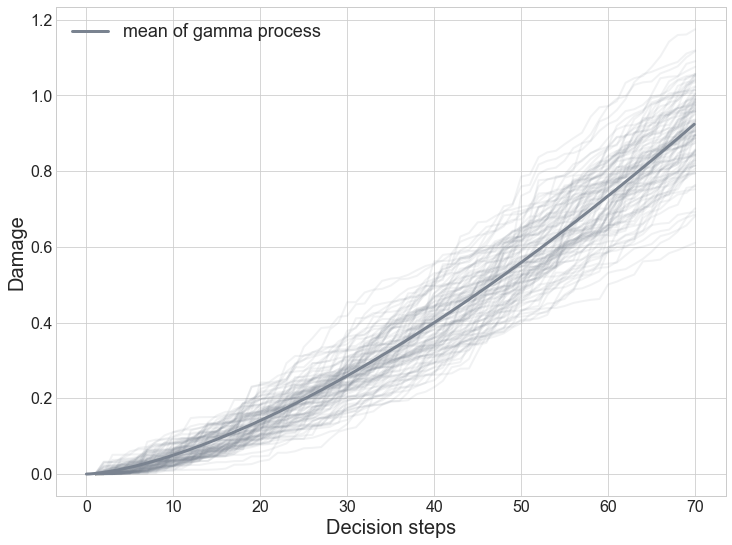
\includegraphics[width=0.7\linewidth]{Figures/gamma.png}
	\caption{Non stationary Gamma process describing the damage evolution over 70 years}
	\label{gamma}
\end{figure}


%------------------------------------------------------------------------------
%	RESEARCH GAP
%------------------------------------------------------------------------------


\subsection{Research gap}

Throughout the literature review, a plethora of obstacles and features that needed improvement was noted, enriching the existing research gap and shaping the final research question and problem formulation. \\

As a general observation, the majority of the examined papers, considers only discrete deterioration states, owing to the computational complexity that is induced in continuous or large state-spaces. This necessity for an efficient maintenance framework for large/continuous state spaces is highlighted in \cite{compare2018markov}, \cite{papakonstantinou2014planning2}.\\

What is more, a common assumption in many papers is full observability of the environment, and consequently not accounting for measurement errors. This issue is being mentioned as a future improvement in \cite{compare2018markov}, \cite{memarzadeh2019model} and \cite{rocchetta2019reinforcement}. Additionally, while the framework proposed in \cite{hausknecht2015deep} considers a \gls{POMDP}, its efficiency is low when observability is low, emphasizing the need of an efficient integration of Bayesian Inference.\\

One of the few cases when a large and continuous state space was considered, along with \gls{DQN}, is in \cite{rocchetta2019reinforcement}. However, the authors stressed out the need of including partial observability, in the sense of noisy observations, as well as model updating.\\

Lastly, in many papers in which \glspl{POMDP} were considered for stochastic optimal control, it was pointed out that a more efficient algorithm needs to be used. To be more precise, in \cite{andriotis2021value} it is mentioned that instead of point-based algorithms, a more advanced learning technique should be used, making \gls{DRL} the suitable choice. In \cite{morato2022optimal}, where Bayesian Networks and point-based solvers are used, it is also stated that a \gls{DRL} approach to solve Bayesian Updating is necessary. Lastly, in \cite{zhou2022maintenance}, \gls{HCRL} is proposed for the maintenance of large-scale multi-component systems, however, it also refers to the development of a \gls{DRL} algorithm for maintenance as a future improvement.

%------------------------------------------------------------------------------
%	CONCLUSIONS
%------------------------------------------------------------------------------


\subsection{Conclusions}

Concluding this chapter, along with the introduction of various scientific fields, a thorough investigation of the existing literature was presented. Through the findings and comments of other researchers, the advantages and disadvantages of different algorithms were better understood, while at the same time assisted to the choice of the necessary tools for the current project, which will be presented in detail in the coming chapter (Chapter \ref{workflow}) as parts of the general methodology. A significant finding of the literature review constitutes the definition of the existing gap, which was also elaborated extensively, as it further compliments the objective of this thesis and its~contribution.